\documentclass[10pt,a4paper]{article}
\usepackage[utf8]{inputenc}
\usepackage[T1]{fontenc}
\usepackage[polish]{babel}
\let\babellll\lll
\let\lll\relax
\usepackage{polski}
\usepackage{graphicx}
\usepackage{todonotes}
\usepackage{listings}
\usepackage{caption}
\usepackage[backend=biber]{biblatex}

\usepackage[unicode,breaklinks,pdfusetitle,colorlinks=true]{hyperref}
\hypersetup{pdfproducer={Latex with hyperref},pdfcreator={pdflatex},allcolors=[rgb]{0,0,0.4}}
\addto\captionspolish{\renewcommand{\figurename}{Ilustracja}}

\author{Rafał Kabaciński}
\title{Technologie informacyjne\\Wprowadzenie do \LaTeX a}

\newcommand{\zadanie}[1]{\todo[inline,color=teal!20]{Zadanie: #1}}
\newcommand{\uwaga}[1]{\todo[inline,color=red!30]{Uwaga: #1}}

\lstset{
	literate=%
	{ą}{{\k{a}}}1
	{Ą}{{\k{A}}}1
	{ć}{{\'c}}1
	{Ć}{{\'{C}}}1
	{ę}{{\k{e}}}1
	{Ę}{{\k{E}}}1
	{ł}{{\l{}}}1
	{Ł}{{\L{}}}1
	{ń}{{\'n}}1
	{Ń}{{\'N}}1
	{ó}{{\'o}}1
	{Ó}{{\'O}}1
	{ś}{{\'s}}1
	{Ś}{{\'S}}1
	{ż}{{\.z}}1
	{Ż}{{\.Z}}1
	{ź}{{\'z}}1
	{Ź}{{\'Z}}1
}

\addbibresource{bibliografia.bib}

\begin{document}
	\maketitle
	\tableofcontents
	\section{Czym jest \LaTeX}
	\LaTeX jest zestawem makr dla języka i kompilatorów \TeX . Z punktu widzenia użytkownika jest to język znaczników, jak HTML, czy XML, czyli język pozwalający zapisać nie tylko treść dokumentu ale również jego wygląd. W porównaniu do edytorów WYSIWYG (ang. what you see is what you get) pozwala na uzyskanie większej kontroli nad wyglądem dokumentu, oraz wymusza nadanie jednolitej struktury. Dzięki temu łatwe jest pisanie spójnych stylistycznie dokumentów oraz zautomatyzowane tworzenie różnego typu spisów, lub odnośników. Wadą takiego podejścia do pisania dokumentów jest często duży nakład pracy potrzebny do głębokiego zmodyfikowania, lub przygotowania nowego stylu.
	
	Więcej informacji na temat \LaTeX a można znaleźć w następujących źródłach:
	\begin{itemize}
		\item bezpłatny podręcznik, w języku angielskim: \cite{lshort2e},
		\item polskie tłumaczenie powyższego podręcznika: \cite{lshort2ePL},
		\item polski podręcznik na portalu WikiBooks: \cite{WikiBook},
		\item dokumentacja portalu Overleaf: \cite{overleaf}.
	\end{itemize}
	
	
	\section{Rozpoczęcie pracy w \LaTeX u}
	Dokumenty w \LaTeX u pisane są w osobnym pliku, nazywanym plikiem źródłowym, względem dokumentu wynikowego. Aby uzyskać plik wynikowy w żądanym formacie, jak na przykład \textit{pdf}, konieczna jest kompilacja pliku źródłowego.
	
	\zadanie{W instrukcji pojawiać się będą bloki takie jak ten, w których będą umieszczone zadania do wykonania. Prawidłowe wykonanie wszystkich poleceń pozwoli wygenerować dokument taki sam jak załączony do poniższej instrukcji dokument przykładowy.}
	
	\subsection{Struktura dokumentu}
	Pliki źródłowe \LaTeX a muszą składać się z \emph{preambuły} i \emph{ciała} dokumentu. We współczesnych edytorach można znaleźć kreatory pozwalające wstawić gotową strukturę bez konieczności samodzielnego wpisywania wszystkich elementów. Na ilustracji \ref{rys:TS:kreator1} zaprezentowano gdzie można znaleźć taki kreator w programie TeXstudio.
	
	\begin{figure}[h!]
		\centering
		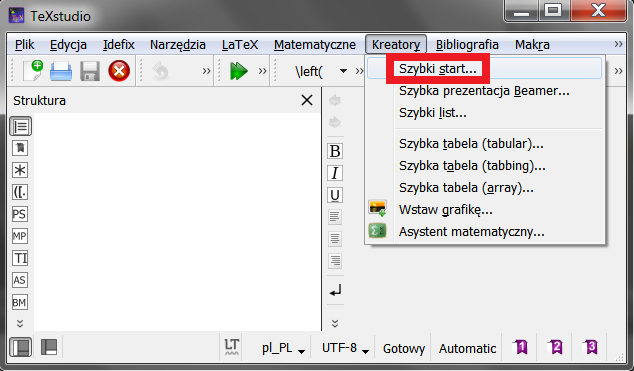
\includegraphics[width=1\textwidth]{Ilustracje/TeXstudio_Kreator1.png}
		\caption{Umiejscowienie kreatora dokumentów w programie TeXstudio}
		\label{rys:TS:kreator1}
	\end{figure}
	
	Po uruchomieniu kreatora pojawia się okno zaprezentowane na ilustracji \ref{rys:TS:kreator2}
	
	\begin{figure}[h!]
		\centering
		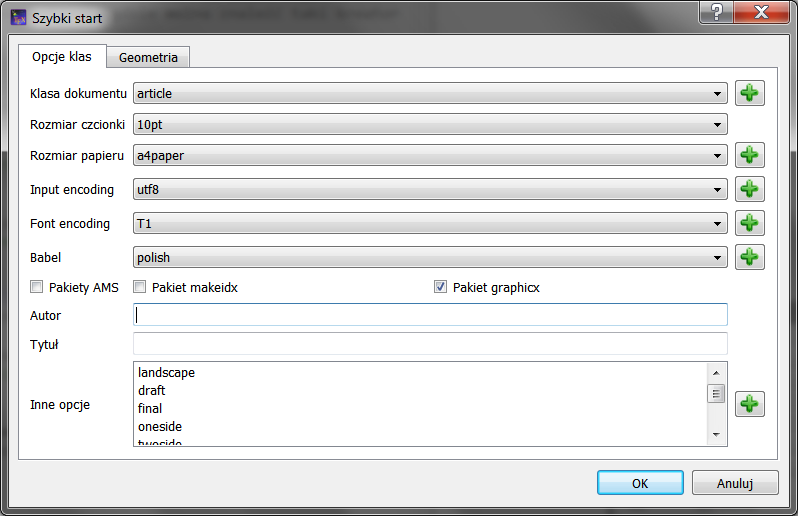
\includegraphics[width=1\textwidth]{Ilustracje/TeXstudio_Kreator2.png}
		\caption{Okno kreatora dokumentów w programie TeXstudio}
		\label{rys:TS:kreator2}
	\end{figure}
	
	\zadanie{Utwórz nowy dokument za pomocą kreatora w programie TeXstudio korzystając z ustawień jak na ilustracji \ref{rys:TS:kreator2}}
	
	Preambuła to wszystko co rozpoczyna się od komendy \lstinline|\documentclass| i kończy na komendzie \lstinline|\begin{document}|. Ciało dokumentu zawiera się wewnątrz otoczenia \lstinline|document|, czyli znajduje się pomiędzy komendami \lstinline|\begin{document}| a \lstinline|\end{document}|. W preambule definiuje się styl dokumentu i dodaje pakiety rozszerzeń. Dobrą praktyką jest definiowanie nowych komend tylko w preambule, ale nie jest to wymagane. Ciało dokumentu zawiera treść wraz ze znacznikami formatowania. Nie można wprowadzać tekstu poza ciałem dokumentu, przeważnie uniemożliwi to kompilację.
	
	Główne okno TeXstudio zaprezentowano na ilustracji \ref{rys:TS:Okno}. W jego skład wchodzi pasek menu i narzędzi (domyślnie u góry), panel boczny (domyślnie po lewej), okno edytora (domyślnie po środku), okno komunikatów (domyślnie na dole) i okno podglądu (domyślnie po prawej). Aby skompilować dokument należy kliknąć przyciski oznaczone pojedynczą bądź podwójnym zielonym trójkątem (patrz ilustracja \ref{rys:TS:Kompilacja}). Ikona z pojedynczym trójkątem oznacza samą kompilację, natomiast z podwójnym kompilację i podgląd.
	
	\uwaga{aby pojawił się podgląd dokument musi zostać skompilowany z powodzeniem. Jeżeli ciało dokumentu jest puste dokument nie zostanie skompilowany.}
	\uwaga{Okno podglądu pokazuje wynik ostatniej udanej kompilacji. Informację czy kompilacja zakończyła się powodzeniem można znaleźć w oknie komunikatów!}
	
	\begin{figure}[h!]
		\centering
		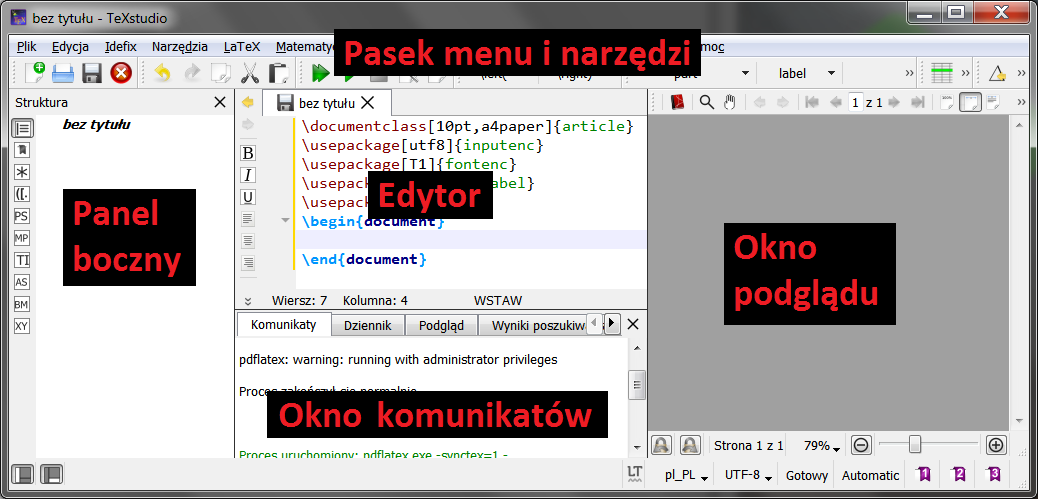
\includegraphics[width=1\textwidth]{Ilustracje/TeXstudio_Okno1.png}
		\caption{Okno programu TeXstudio}
		\label{rys:TS:Okno}
	\end{figure}
	
	\begin{figure}[h!]
		\centering
		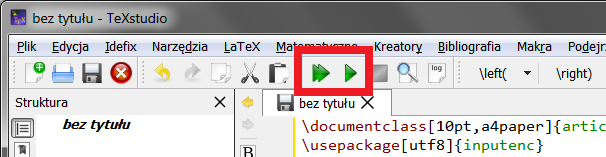
\includegraphics[width=1\textwidth]{Ilustracje/TeXstudio_kompilacja.png}
		\caption{Przyciski kompilacji w programie TeXstudio}
		\label{rys:TS:Kompilacja}
	\end{figure}

	Preambuła wstawiona przez edytor zawiera od razu kilka pakietów. Pierwszym z nich jest pakiet \lstinline|\usepackage[utf8]{inputenc}| informujący kompilator o kodowaniu pliku źródłowego. Po utworzeniu pliku nie należy zmieniać oznaczenia kodowania, gdyż uniemożliwi to kompilację dokumentu! 

	\zadanie{Skompiluj z powodzeniem swój pierwszy dokument w \LaTeX u.}
	
	\uwaga{\LaTeX jest zbiorem wielu osobnych programów, wymieniających ze sobą informacje za pomocą plików tymczasowych pojawiających się w tym samym folderze co plik kompilowany. Z tego względu dobrą praktyką jest umieszczanie tych dokumentów w osobnych folderach.}
	
	\subsection{Komendy w \LaTeX u}
	
	Komenda w \LaTeX u składa się z ukośnika wstecznego: ,,$\backslash$'' i ciągu literowo--cyfrowego, każdy inny znak w tym spacje przerywa komendę. Jeżeli komenda przyjmuje argumenty obowiązkowe znajdują się one pomiędzy znakami nawiasów klamrowych: ,,\{\}''. Argumenty opcjonalne umieszczane są w nawiasach kwadratowych: ,,[]''. Kolejność występowania nawiasów zależy od komendy, dlatego warto korzystać z podpowiedzi oferowanych przez współczesne edytory. Przykład takich podpowiedzi zaprezentowano na ilustracji \ref{rys:TS:Podpowiedzi}. Wyboru wariantu dokonuje się strzałkami na klawiaturze i potwierdza klawiszem \emph{enter}.
	
	\begin{figure}[h!]
		\centering
		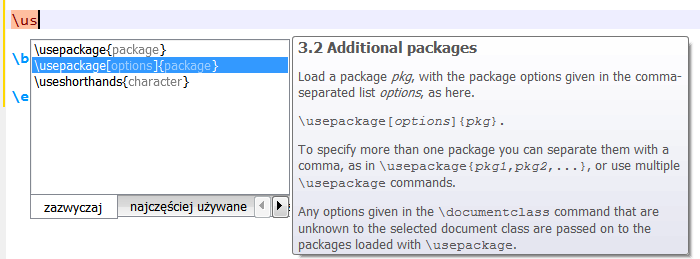
\includegraphics[width=1\textwidth]{Ilustracje/TeXstudio_podpowiedzi.png}
		\caption{Podpowiedzi w edytorze TeXstudio}
		\label{rys:TS:Podpowiedzi}
	\end{figure}
	
	\subsection{Pisanie dokumentów w języku polskim}
	
	Drugim pakietem wstawionym przez kreator jest \lstinline|\usepackage[T1]{fontenc}| informujący kompilator o kodowaniu czcionek w dokumencie wynikowym. Dla języka polskiego prawidłowym zestawem jest \emph{T1}. Brak tego pakietu lub ustawienie niewłaściwej opcji spowoduje błędy w kompilacji lub wstawienie niewłaściwych liter w miejsce polskich znaków diakrytyzowanych. Trzecim pakietem jest pakiet \lstinline|\usepackage[polish]{babel}|. Pakiet ten pozwala na dostosowanie między innymi podziału słów między wierszami według reguł języka polskiego. Oprócz powyższych warto dodać jeszcze trzeci pakiet: \lstinline|\usepackage{polski}|, dostosowujący pozostałe aspekty \LaTeX a.
	
	\zadanie{Dodaj, korzystając z podpowiedzi edytora, pakiet polski i skompiluj dokument.}
	
	\uwaga{Pakiety w \LaTeX u są pisane przez niezależnych autorów i może między nimi dochodzić do konfliktów. Czasem pakiety są w stanie koegzystować bez konieczności ingerencji w ich makra, o ile są dodane w określonej kolejności. Przykładem jest pakiet \emph{babel} z opcją \emph{polish} i pakiet \emph{amssymb}. Jeżeli pakiet AMS jest dodany przed pakietem babel dokument można skompilować, w odwrotnej kolejności prowadzi to do błędu. Najbezpieczniejszą strategią jest dodawanie nieznanych pakietów pojedynczo.}

	 
	\section{Podstawy pisania dokumentów w \LaTeX u}
	\subsection{Tytuł i autor}
	
	Elementy należące do struktury dokumentu, takie jak na przykład jego tytuł nie powinny być formatowane wprost lecz należy skorzystać z odpowiednich funkcji do ich wywołania. Aby zdefiniować zawartość tytułu należy użyć poleceń:
	\begin{itemize}
		\item \lstinline|\title{}| -- definiuje tytuł dokumentu,
		\item \lstinline|\author{}| -- definiuje autora/autorów,
		\item \lstinline|\date{}| -- zmienia datę pod tytułem.
	\end{itemize}
	\zadanie{zdefiniuj tytuł i autora swojego dokumentu i go skompiluj. Czy tytuł się pojawił?}
	Powyższe komendy definiują zawartość powyższych pól w dokumencie ale nie wstawiają samego tytułu. Poleceniem, które umieści tytuł jest komenda:
	\begin{lstlisting}
		\maketitle
	\end{lstlisting}
	Tytuł pojawi się w dokumencie w miejscu wywołania tego polecenia. Komenda \lstinline|\date{}| różni się od pozostałych, gdyż nawet przy braku zdefiniowanej daty zostanie wstawiona data kompilacji. Polecenia tego używa się gdy konieczna jest zmiana daty.
	\zadanie{Skompiluj dokument z tytułem}
	
	
	\subsection{Spis treści}
	\zadanie{Od tego momentu nie kompiluj dokumentu dopóki nie pojawi się takie polecenie w  zadaniu}
	
	Jedną z głównych zalet \LaTeX a jest zautomatyzowane tworzenie list takich jak spis treści. Dostępne są następujące poziomy podziału dokumentu:
	\begin{itemize}
		\item \lstinline|\part{tytuł}| -- część,
		\item \lstinline|\chapter{tytuł}| -- rozdział, dostępny tylko w dokumentach typu książka (book) i raport (report),
		\item \lstinline|\section{tytuł}| -- sekcja,
		\item \lstinline|\subsection{tytuł}| -- podsekcja,
		\item \lstinline|\subsubsection{tytuł}| -- podpodsekcja,
		\item \lstinline|\paragraph{tytuł}| -- paragraf,
		\item \lstinline|\subparagraph{tytuł}| -- podparagraf.
	\end{itemize}
	W dokumentach typu list (letter) nie są dostępne żadne stopnie podziału.
	
	Komendą jaka wstawia spis treści do dokumentu jest:
	\begin{lstlisting}
		\tableofcontents
	\end{lstlisting}
	Polecenie to wstawi spis treści w miejscu w którym zostanie umieszczone w ciele dokumentu.
	\zadanie{Umieść w swoim dokumencie polecenie \emph{tableofcontents} i przepisz pierwsze dwie sekcje z dokumentu przykładowego. Dopiero wtedy skompiluj dokument. Do tytułu jednej z sekcji dopisz losową literę i skompiluj dokument jeszcze raz. Gdzie pojawiła się losowa litera dopisana do tytułu? Czy kolejna kompilacja rozwiązuje problem?}
	
	W tytułach sekcji w dokumencie przykładowym wykorzystano logo \LaTeX a. Poleceniem wstawienia takiego loga jest \lstinline|\LaTeX|.
	\uwaga{Nazwy poleceń w \LaTeX u są wrażliwe na wielkość liter! polecenie \emph{LaTeX} to nie to samo co \emph{latex}!}
	\zadanie{Wstaw loga \LaTeX do swoich tytułów sekcji. Czy wyglądają tak jak w dokumencie przykładowym?}
	\LaTeX\ ignoruje białe znaki po komendach. Jeżeli potrzebna jest spacja po komendzie należy użyć polecenia wstawienia spacji: ,,\lstinline|\ |''.
	
	
	\subsection{Otoczenia}
	
	Ważnym elementem \LaTeX a są tak zwane otoczenia. Przeważnie korzystają one z konstrukcji:
	\begin{lstlisting}
		\begin{Nazwa_otoczenia}
			zawartość...
		\end{Nazwa_otoczenia}
	\end{lstlisting}
	Istotną cechą otoczeń jest to, że muszą się nawzajem otaczać, nie mogą się przecinać! W związku z tym niedozwolona jest na przykład taka konstrukcja:
	\begin{lstlisting}
		\begin{Otoczenie1}
			\begin{Otoczenie2}
			
		\end{Otoczenie1}
			\end{Otoczenie2}
	\end{lstlisting}
	
	Przykładem otoczenia jest środowisko do pisania list wypunktowanych:
	\begin{lstlisting}
		\begin{itemize}
			\item Treść punktu 1
			\item Treść punktu 2
		\end{itemize}
	\end{lstlisting}
	Siostrzanym środowiskiem jest otoczenie dla list numerowanych:
	\begin{lstlisting}
		\begin{enumerate}
			\item Treść punktu 1
			\item Treść punktu 2
		\end{enumerate}
	\end{lstlisting}
	\zadanie{Odtwórz w swoim dokumencie listę wypunktowaną z dokumentu przykładowego}
	
	\subsection{Formatowanie tekstu}
	
	W dokumentach pisanych w \LaTeX u nie jest dobrą praktyką aby zmieniać lokalnie formatowanie lub rozmiar czcionek, gdyż prowadzi to do powstania niespójności stylistycznych. Zmian takich należy dokonywać na poziomie stylu całego dokumentu, na przykład poprzez zmianę rozmiaru czcionki w argumencie opcjonalnym polecenia \lstinline|\documentclass[arg. opcjonalne]{typ dokumentu}|.
	
	Czasem konieczne są jednak pewne zmiany, aby wyróżnić pewne fragmenty tekstu i \LaTeX\ udostępnia takie narzędzia:
	\begin{itemize}
		\item \lstinline|\emph{tekst}| -- wyróżnia tekst, sposób wyróżnienia zależny jest od stylu dokumentu,
		\item \lstinline|\textbf{tekst}| -- pogrubia czcionkę,
		\item \lstinline|\textit{tekst}| -- pochyla czcionkę,
		\item \lstinline|\underline{tekst}| -- podkreśla tekst,
	\end{itemize}

	Możliwa jest też lokalne zdefiniowanie rozmiaru tekstu:
	\begin{itemize}
		\item \lstinline|\Huge| -- {\Huge tekst},
		\item \lstinline|\huge| -- {\huge tekst},
		\item \lstinline|\LARGE| -- {\LARGE tekst},
		\item \lstinline|\Large| -- {\Large tekst},
		\item \lstinline|\large| -- {\large tekst},
		\item \lstinline|\normalsize| -- {\normalsize tekst},
		\item \lstinline|\small| -- {\small tekst},
		\item \lstinline|\footnotesize| -- {\footnotesize tekst},
		\item \lstinline|\scriptsize| -- {\scriptsize tekst},
		\item \lstinline|\tiny| -- {\tiny tekst},
	\end{itemize}
	
	\uwaga{Powyższe polecenia zmieniają rozmiar w całym otoczeniu w którym zostaną użyte! Aby ograniczyć ich zasięg należy umieszczać je wraz z tekstem w nawiasach klamrowych.}
	
	\section{Formuły matematyczne}
	
	Język \LaTeX znany jest z bardzo rozbudowanego systemu do składu formuł matematycznych, który wykorzystywany jest w innych środowiskach, jak na przykład Matlab czy Python. Same formuły matematyczne w \LaTeX u muszą być umieszczone w odpowiednich otoczeniach matematycznych których są trzy rodzaje:
	\begin{itemize}
		\item \lstinline|$\sin x$| -- pojedyncze dolary umieszczają formułę w linii wraz z tekstem: $\sin x$
		\item \lstinline|$$\sin x$$| -- podwójne dolary umieszczają formułę w osobnej linii: $$\sin x$$
		\item \lstinline|\begin{equation}\sin x\end{equation}| -- otoczenie \emph{equation} umieszcza formułę w osobnej linii i nadaje jej numer: \begin{equation}\sin x\end{equation}
	\end{itemize}

	Tylko otoczenia \emph{equation} pozwalają na wykorzystanie polecenia \emph{label} i odwołanie się do danej formuły.
	
	\uwaga{Wewnątrz otoczeń matematycznych nie wolno zostawiać pustych linii. Może prowadzić to do nieoczekiwanych błędów!}
	
	Przy pisaniu formuł matematycznych przydatny jest przybornik z symbolami matematycznymi dostępny w programie TeXstudio. Dostęp do niego można uzyskać klikając jego ikonę na panelu bocznym, co zaprezentowano na ilustracji~\ref{rys:TS:Symbole}. Zakres wyświetlanych symboli można ograniczyć przyciskiem z prawej strony panelu.
	
	\begin{figure}[h!]
		\centering
		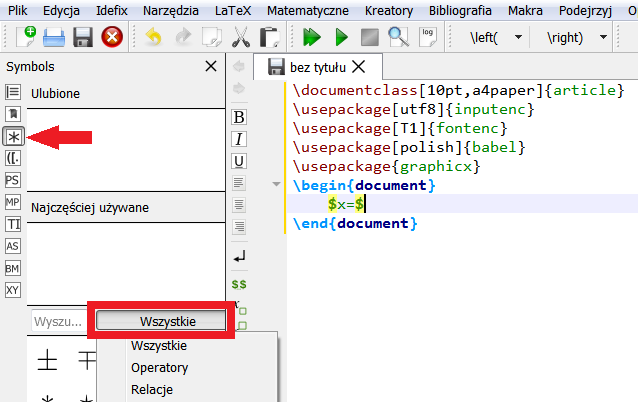
\includegraphics[width=1\textwidth]{Ilustracje/TeXstudio_Symbole.png}
		\caption{Przybornik z symbolami matematycznymi w TeXstudio}
		\label{rys:TS:Symbole}
	\end{figure}
	
	Podstawowe polecenia przydatne przy pisaniu formuł matematycznych:
	\begin{itemize}
		\item \lstinline|$x^{2b}$ | = $x^{2b}$,
		\item \lstinline|$x_{2b}$ | = $x_{2b}$,
		\item \lstinline|$\frac{a}{b}$ | = $\frac{a}{b}$,
		\item \lstinline|$\int i(t) dt$ | = $\int i(t) dt$,
		\item \lstinline|$\int\limits_{-T}^{T}i(t)dt$| = $\int\limits_{-T}^{T} i(t)dt$.
	\end{itemize}
	
	\zadanie{Odwzoruj pierwszy wzór matematyczny z dokumentu do odtworzenia. W jakim otozeniu matematycznym został od zapisany?}
	
	W \LaTeX u nawiasy okrągłe i kwadratowe w formułach matematycznych można stosować wprost: $(),[]$. W przypadku nawiasów klamrowych należy poprzedzić je ukośnikami wstecznymi. Na przykład \lstinline|$\{ \}$|, daje: $\{\}$. Nawiasy takie jednak nie dostosują swoich rozmiarów do zawartości. Aby uzyskać taki efekt należy użyć poleceń \lstinline|\left| i \lstinline|\right|:
	
	 \lstinline|$\left(\frac{a}{b}\right)$| = $\left(\frac{a}{b}\right)$. 
	 
	 Polecenia te tworzą otoczenie nawiasowe, w związku z czym nie mogą się przecinać z innymi otoczeniami. Znaki nawiasów nie muszą sobie odpowiadać, można otworzyć otocznie nawiasem okrągłym i~zamknąć kwadratowym: \lstinline|$\left(\frac{a}{b}\right]$| = $\left(\frac{a}{b}\right]$. Jeżeli nie chcemy aby z którejś strony pojawił się znak nawiasu należy użyć kropki, samo otoczenie musi jednak zostać zamknięte: \lstinline|$\left\{\frac{a}{b}\right.$| = $\left\{\frac{a}{b}\right.$.
	
	Aby odtworzyć drugi wzór z dokumentu przykładowego konieczne będzie otoczenie \emph{array}. Służy ono do definiowania tabel w trybie matematycznym. Przyjmuje ono jeden argument obowiązkowy w którym definiuje się liczbę i~wyjustowanie kolumn. W tym celu dostępne są trzy litery: \emph{l} -- kolumna wyjustowana do lewej,  \emph{c} -- kolumna wyjustowana do środka, \emph{r} -- kolumna wyjustowana do prawej. Do separacji komórek wewnątrz tabeli służy znak ampersand: ,,\&''. Przejście do nowego wiersza jest oznaczone podwójnym ukośnikiem wstecznym: ,,\verb|\\|''. Przykładowo układ 2 na 2 elementy, wyjustowane do środka, będzie zdefiniowany następująco:
	
	\begin{tabular}{cc}
		\begin{lstlisting}
		$\begin{array}{cc}
		a & b \\ c & d
		\end{array}$
		\end{lstlisting}
		&
		$\begin{array}{cc}
		a & b \\ c & d
		\end{array}$
	\end{tabular}
	
	
	\zadanie{Spróbuj odtworzyć wzór na macierz rotacji z dokumentu do odtworzenia.}
	
	\section{Tabele i rysunki}
	
	
	Tabele w trybie tekstowym definiuje się za pomocą otoczenia \emph{tabular}, które  działa tak samo jak otoczenie \emph{array} w trybie matematycznym. Linie oddzielające kolumny uzyskać można wstawiając znak kreski pionowej: ,,|'' między literami definiującymi kolumny. Z kolei linie poziome uzyskuje się za pomocą komendy \lstinline|\hline| pomiędzy wierszami:
	
	\begin{center}
	\begin{tabular}{cc}
		\begin{tabular}{c}
		\begin{lstlisting}
\begin{tabular}{|c|c|}
\hline
a & b \\ \hline
c & d \\ \hline
\end{tabular}
		\end{lstlisting}
		\end{tabular}
		&
		\begin{tabular}{|c|c|}
			\hline a & b \\ \hline
			 c & d \\ \hline
		\end{tabular}
	\end{tabular}
	\end{center}

	Tabela zdefiniowana za pomocą otoczenia \emph{tabular} jest traktowana tak jak tekst i może być wstawiona nawet w środku linii: \begin{tabular}{|c|c|}
		\hline
		a & b \\ \hline
		c & d \\ \hline
	\end{tabular}.
	Aby wyróżnić tabelę z tekstu należy umieścić ją w otoczeniu pływającym \emph{table}:
	\begin{lstlisting}
\begin{table}
	\begin{tabular}{|c|c|}
		\hline
		a & b \\ \hline
		c & d \\ \hline
	\end{tabular}
\end{table}
	\end{lstlisting}
	
	\zadanie{Zdefiniuj własną tabelę w otoczeniu pływającym. Gdzie się pojawiła w dokumencie po kompilacji?}
	
	Otoczenia pływające przyjmują argument opcjonalny informujący o pożądanym położeniu. Dostępne są następujące litery:
	\begin{itemize}
		\item h -- w miejscu w którym jest w kodzie,
		\item t -- u góry strony,
		\item b -- na dole strony,
		\item p -- na osobnej stronie z tabelami,
	\end{itemize}
	Powyższe argumenty są jednak jedynie sugestiami, a tabela może zostać umieszczona dowolnie. Znak wykrzyknika za parametrem położenia pozwala dodatkowo poluzować ustawienia \LaTeX a, ale nadal nie jest bezwzględnym nakazem. Przykład:
	
	\begin{lstlisting}
\begin{table}[h!]
	\begin{tabular}{|c|c|}
	a & b \\ \hline
	c & d \\ \hline
	\end{tabular}
\end{table}
	\end{lstlisting}
	\zadanie{Sprawdź czy dodanie parametru położenia przeniesie Twoją tabelę w prawidłowe miejsce.}
	
	Wewnątrz otoczeń pływających, do opisu zawartości, służy polecenie \lstinline|\caption{}|:
	
	\begin{lstlisting}
\begin{table}[h!]
\caption{Przykład}
	\begin{tabular}{c|c}
		a & b \\ \hline
		c & d
	\end{tabular}
\end{table}
	\end{lstlisting}

	Otoczeniem pływającym dla ilustracji jest otoczenie \emph{figure}. Same ilustracje można wstawić za pomocą polecenia:
	
	\begin{lstlisting}
\includegraphics[argumenty opcjonalne]{ścieżka do pliku}|
	\end{lstlisting}
	
	 Ścieżki do pliku mogą być względne lub bezwzględne. Zalecane jest umieszczanie plików z rysunkami w tym samym folderze co kompilowany plik, lub podfolderze i podanie ścieżki względnej:
	
	\begin{lstlisting}

\includegraphics{Rys/pp-putlogopelne.png}
	\end{lstlisting}
	
	Foldery oddziela się znakiem ukośnika: ,,/''. W celu wyjustowania rysunku do środka można użyć polecenia \lstinline|\centering|, które wyśrodkuje wszystko wewnątrz otoczenia w którym zostało użyte. Aby zmienić rozmiar rysunku, należy wpisać polecenie: \lstinline|width=0.5\textwidth|, które dostosuje szerokość rysunku do połowy szerokości tekstu:
	
	\begin{lstlisting}
\begin{figure}[h!]
	\centering
	
\includegraphics[width=0.5\textwidth]
	{Rys/pp-putlogopelne.png}
	\caption{Przykładowy rysunek}
\end{figure}
	\end{lstlisting}
	
	Aby odwołać się w dokumencie do danego rysunku bądź tabeli pod poleceniem \lstinline|\caption{}| należy umieścić polecenie \lstinline|\label{etykieta}|. Następnie w miejscu w którym ma pojawić się odwołanie należy umieścić polecenie \lstinline|\ref{etykieta}|.
	
	\zadanie{Odtwórz rysunek i tabelę z dokumentu przykładowego wraz z odwołaniami.}
	
	\section{Kod źródłowy w dokumentach}
	
	Aby wpisać kod źródłowy do dokumentu można skorzystać z podstawowego polecenia \verb/\verb|kod|/. Pozwala ono na wpisanie kodu, który nie będzie interpretowny przez \LaTeX a i będzie wyróżniony z tekstu. Wypisywan jest on za pomocą czcionki o stałej szerokości. Komenda ta pozwala jednak na wstawienie tylko pojedynczej linijki kodu. W przypadku bardziej rozbudowanego źródła, lub potrzeby kolorowania składni, dodać należy pakiet \verb|\usepackage{listings}|. Jezyk dla którego ma być kolorowana składnia można ustawić za pomocą polecenia: \verb|\lstset{language=C++}| lub w argumentach opcjonalnych otoczenia z wstawianym kodem:
	
	\hspace{0.15\textwidth}
	\begin{minipage}{0.75\textwidth}
		\noindent\verb|\begin{lstlisting}[language=C++]|\\
		\verb|for(int i=0;1<10;i++){}|\\
		\verb|\end{lstlisting}|
	\end{minipage}

	Możliwe jest też wstawienie do dokumentu całego pliku z kodem źródłowym:
	
	\verb|\lstinputlisting[language=C++]{plik.cpp}|
	
	\zadanie{Przepisz kod źródłowy z przykładowego dokumentu, wraz z właściwym kolorowaniem, składni.}
	
	%\section{Overleaf}
	%Overleaf - praca kolaboracyjna, obsługa, pułapki.
	
	%\section{Dla zainteresowanych}
	
	\printbibliography
	
\end{document}